\documentclass[11pt]{article}

% ===== SODA 2027 submission (full version). 11pt, single-column, 1-inch margins, letter. =====
% Lightweight double-blind: anonymized from day 1 (no author/affiliation/self-citation tells).

\usepackage[letterpaper,margin=1in]{geometry}
\usepackage{amsmath,amssymb,amsthm,mathtools}
\usepackage{microtype}
\usepackage[dvipsnames]{xcolor}
\usepackage{enumitem}
\usepackage{booktabs}
\usepackage[ruled,vlined]{algorithm2e}
\usepackage{tikz}
\usetikzlibrary{arrows.meta,positioning,calc,patterns}
\usepackage{hyperref}
\hypersetup{colorlinks=true,linkcolor=blue!50!black,citecolor=green!40!black,urlcolor=blue!60!black}
\usepackage[capitalize,nameinlink]{cleveref}

% ===== Shared macros (keep consistent; never inline a symbol that has a macro) =====
\newcommand{\eps}{\varepsilon}
\newcommand{\R}{\mathbb{R}}
\newcommand{\Z}{\mathbb{Z}}
\newcommand{\N}{\mathbb{N}}
\newcommand{\E}{\mathbb{E}}
\newcommand{\Var}{\operatorname{Var}}
\newcommand{\Prob}{\Pr}
\newcommand{\MST}{\mathrm{MST}}
\newcommand{\wt}{w}                         % weight of a tree / edge
\newcommand{\Otil}{\widetilde{O}}
\newcommand{\Wq}{W_Q}                        % w(MST(Q))
\newcommand{\diam}{\operatorname{diam}}
\newcommand{\dist}{\operatorname{dist}}
\newcommand{\cQ}{c_Q}                        % component count of Q's threshold graph
\newcommand{\cG}{c_\Gamma}                   % component count of the scale graph
\newcommand{\eqdef}{\vcentcolon=}
\newcommand{\given}{\mid}
\newcommand{\poly}{\operatorname{poly}}
\newcommand{\sgn}{\operatorname{sgn}}
\newcommand{\set}[1]{\left\{#1\right\}}
\newcommand{\abs}[1]{\left|#1\right|}
\newcommand{\floor}[1]{\left\lfloor #1 \right\rfloor}
\newcommand{\ceil}[1]{\left\lceil #1 \right\rceil}
\newcommand{\norm}[1]{\left\lVert #1 \right\rVert}
% range-counting oracle
\newcommand{\rcount}[1]{\mathsf{count}(#1)}
\newcommand{\Range}{\mathcal{R}}
\newcommand{\rep}{\operatorname{rep}}            % WSPD cell representative


% ===== Theorem environments =====
\theoremstyle{plain}
\newtheorem{theorem}{Theorem}
\newtheorem{lemma}{Lemma}
\newtheorem{proposition}{Proposition}
\newtheorem{corollary}{Corollary}
\theoremstyle{definition}
\newtheorem{definition}{Definition}
\newtheorem{remark}{Remark}
\newtheorem{problem}{Problem}
\theoremstyle{plain}
\newtheorem*{theorem*}{Theorem}
\newtheorem*{lemma*}{Lemma}
\newtheorem*{corollary*}{Corollary}

\title{Estimating Euclidean MST Weight in\\ $\widetilde{O}(n^{1/3})$ Range-Counting Queries}
\author{}
\date{}

\begin{document}
\maketitle

\begin{abstract}
% WRITTEN LAST (W1 order). Placeholder.
We study the estimation of the Euclidean minimum spanning tree (MST) weight of $n$ points in $[\Delta]^2$
($\Delta=O(n)$) under an orthogonal range-counting oracle, which returns the number of input points in a
query rectangle and is the native primitive of a spatial index. We give a randomized algorithm that
$(1\pm\eps)$-estimates the MST weight using $\Otil_\eps(n^{1/3})$ range-counting queries, and runs in time
near-linear in its query count. This matches the $\Omega(n^{1/3})$ lower bound of Driemel et al.\ (SoCG
2025) up to polylogarithmic and $\eps$-dependent factors, settling the polynomial query exponent of
Euclidean MST-weight estimation in this model and improving the previous $\Otil(\sqrt n)$ upper bound to
the tight rate.

The improvement comes from one new primitive, an \emph{empty-cell spatial leader estimator} for the number
of connected components of an implicitly defined geometric graph. Where the natural approach samples points
and pays $\Omega(\sqrt n)$ to see the rare heavy clusters that carry most of the weight, our estimator
samples grid cells from a universe that includes empty ones, so a heavy cluster is found in proportion to
the space it occupies and not its (small) mass; its variance is governed by the component count, and an
active-cover packing inequality then collapses the per-scale costs to $\Otil(\sqrt K)$ on a support of $K$
cells. Combined with a clipped death-time sampler for the bulk of the weight and a support
regularization that routes the heavy tail through a snapped grid, balancing at $K=\Theta(n^{2/3})$ yields
the $n^{1/3}$ rate.

\end{abstract}

\section{Introduction}\label{sec:intro}

% WRITTEN LATE (contributions map 1:1 to existing theorems). Stub with subsection skeleton. [TODO]

% 1.1 Our results: Thm~\ref{thm:main} (Otil(n^{1/3})) + Lem~\ref{lem:support} + tightness corollary;
%     prior-bound comparison table (Czumaj'05 / Driemel UB / Driemel LB / ours).
\subsection{Our results}\label{sec:intro-results}
% [TODO]

% 1.2 Techniques: empty-cell spatial leader estimator (the new primitive); support regularization +
%     snapping; range-counting clipped death-time; the cluster-count integral (CRT lineage).
\subsection{Techniques}\label{sec:intro-tech}
% [TODO]

% 1.3 Related work folded HERE (not a late standalone section): sublinear MST (CRT, Patlin-vdB,
%     Czumaj-Sohler), range-counting oracles (Driemel et al.), single-linkage clustering cost
%     (Peng-Sohler-Xu), WSPD/spanners, distance-oracle MST, streaming EMST.
\subsection{Related work}\label{sec:intro-related}
% [TODO]

\section{Technical overview}\label{sec:overview}

This section walks through the whole argument at the level of ideas, so that the formal development in
\cref{sec:support,sec:dt,sec:main} and the proofs in the appendices can be read against a map. Nothing
here is used later; the reader who prefers to start from definitions may skip to \cref{sec:prelim}.

\subsection{The cluster-count integral and where the cost hides}\label{sec:ov-integral}

Every sublinear MST-weight algorithm in this lineage rests on one identity. For a finite $S\subset\R^2$
and a threshold $t$, let $c_S(t)$ be the number of connected components of the graph that joins two points
of $S$ when they are within distance $t$; these components are the single-linkage clusters at scale $t$.
As $t$ grows the clusters merge, each merge corresponding to one MST edge, and the Chazelle--Rubinfeld--
Trevisan identity~\cite{CRT05} writes the MST weight as the area under the resulting staircase,
\begin{equation}\label{eq:ov-integral}
  \wt(\MST(S))=\int_0^\infty\bigl(c_S(t)-1\bigr)\,dt .
\end{equation}
Estimating $\wt(\MST(S))$ thus reduces to estimating the curve $c_S(\cdot)$ at a geometric ladder of
thresholds and summing. Under the range-counting oracle we cannot see points, only counts in boxes, so the
whole problem becomes: \emph{estimate the number of single-linkage clusters at a given scale, using few
range counts.}

Counting components in sublinear time is classically done by sampling: pick a few vertices, explore their
components, and extrapolate~\cite{CRT05,CzumajSohler09}. In the geometric setting this is exactly what
costs $\Omega(\sqrt n)$. The reason is a mismatch between mass and weight. Consider a dense
$\sqrt K\times\sqrt K$ block of points together with a handful of far-flung satellites. The satellites are
a vanishing fraction of the points, so a sample of $\poly\log$ many points misses them with high
probability; yet each satellite is its own cluster across a wide range of scales and so contributes a
constant fraction of the MST weight. To see the satellites by sampling \emph{points} one must draw
$\Omega(\sqrt K)$ of them, and paying this at every scale is the $\sqrt n$ barrier of~\cite{DMOSW25}.

\subsection{The empty-cell spatial leader estimator}\label{sec:ov-leader}

Our one new primitive removes that barrier by sampling \emph{space} instead of mass. Fix a scale and lay
down a fine grid. Form the \emph{scale graph} whose vertices are the nonempty cells and whose edges join
cells that are close, so that its component count brackets $c_S$ at nearby thresholds
(\cref{sec:support-filtration}). To estimate the number of components $c$ of a graph $\Gamma$ on a known
universe $\mathcal U$ of $M$ candidate cells, run the following one-bit experiment, illustrated in
\cref{fig:leader}.

\begin{quote}
Draw a cell $X$ uniformly from $\mathcal U$, \emph{including empty cells}. If $X$ is empty, output $Z=0$.
Otherwise assign independent uniform ranks to the occupied cells and explore the component of $X$ in
$\Gamma$, stopping as soon as a cell of smaller rank than $X$ appears. Output $Z=M$ if $X$ is the
minimum-rank cell of its component (its \emph{leader}) and $Z=0$ otherwise.
\end{quote}

\begin{figure}[t]
\centering
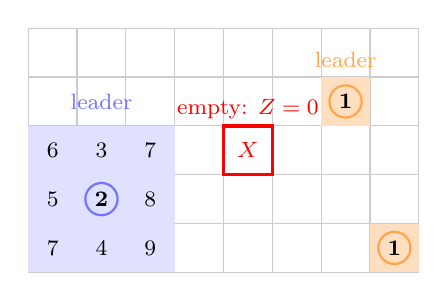
\begin{tikzpicture}[scale=0.62, every node/.style={font=\footnotesize}]
  % grid
  \draw[step=1cm, gray!40, thin] (0,0) grid (8,5);
  % a dense block (occupied cells) bottom-left
  \foreach \x/\y in {0/0,1/0,2/0,0/1,1/1,2/1,0/2,1/2,2/2} {
    \fill[blue!12] (\x,\y) rectangle (\x+1,\y+1);
  }
  % ranks in the block component (min-rank = leader)
  \node at (0.5,0.5) {7}; \node at (1.5,0.5) {4}; \node at (2.5,0.5) {9};
  \node at (0.5,1.5) {5}; \node at (1.5,1.5) {\textbf{2}}; \node at (2.5,1.5) {8};
  \node at (0.5,2.5) {6}; \node at (1.5,2.5) {3}; \node at (2.5,2.5) {7};
  \draw[blue!55,thick] (1.5,1.5) circle (0.33); % leader of the block
  % two satellites, each its own component
  \fill[orange!25] (6,3) rectangle (7,4); \node at (6.5,3.5) {\textbf{1}};
  \draw[orange!70,thick] (6.5,3.5) circle (0.33);
  \fill[orange!25] (7,0) rectangle (8,1); \node at (7.5,0.5) {\textbf{1}};
  \draw[orange!70,thick] (7.5,0.5) circle (0.33);
  % a sampled empty cell (X)
  \draw[red,very thick] (4,2) rectangle (5,3); \node[red] at (4.5,2.5) {$X$};
  \node[red] at (4.5,3.35) {empty: $Z=0$};
  \node[blue!55] at (1.5,3.5) {leader};
  \node[orange!70] at (6.5,4.35) {leader};
\end{tikzpicture}
\caption{The empty-cell leader estimator. Candidate cells are sampled uniformly from a universe that
includes empty ones (an empty sample, shown in red, returns $0$). On an occupied sample, ranks are drawn
and the unique minimum-rank cell of each component (circled) returns $Z=M$. A far satellite is one cell of
the universe like any other, so it is found with the right probability; its tiny mass never enters.}
\label{fig:leader}
\end{figure}

For any fixed ranking exactly one cell per component is its leader, so exactly $c$ of the $M$ candidates
return $M$ and the rest return $0$. Hence $\E Z=M\cdot(c/M)=c$ and $\E Z^2=M^2\cdot(c/M)=Mc$, giving the
variance bound
\begin{equation}\label{eq:ov-var}
  \E Z=c,\qquad\Var(Z)=Mc-c^2\le Mc .
\end{equation}
Two features make this the right estimator. First, its variance is governed by the \emph{component count}
$c$, not by the number of occupied cells: the satellite is one candidate among $M$ and is sampled with
probability $1/M$ regardless of how few points it holds, so the heavy tail is no longer invisible.
Second, an occupied exploration is cheap in expectation: the cell examined $j$-th in the rank order is
examined only when the start has the smallest rank among the first $j$, an event of probability $1/(j-1)$,
so an exploration touches $O(\log K)$ cells on average, the same harmonic bound that later controls the
death-time search.

\subsection{Two costs, one packing inequality, and the \texorpdfstring{$\sqrt K$}{sqrt K} bound}
\label{sec:ov-twopart}

To turn \eqref{eq:ov-var} into an algorithm we estimate $c=c_\Gamma(r)$ at each scale $r$ to an additive
accuracy $\alpha_r$ tuned so the scale-by-scale errors sum to $\eps\Wq$. A median-of-means average of the
one-bit experiment needs $O(MU/\alpha_r^2)$ trials, where $U\ge c$ is an a-priori bound on the component
count; this is the \emph{trial cost}. Separately, each occupied trial explores cells, and an exploration
can touch up to $N$ occupied cells; this is the \emph{exploration cost}. The crucial point is that these
two costs scale with different quantities, $U$ (a bound on the component count) and $N$ (the occupied-cell
count), and we account for them separately.

Both sums are collapsed by a single geometric fact about the support, the \emph{active-cover packing}
inequality $\Wq\ge b\delta/16$ (\cref{lem:packing}), where $b=\Theta(\sqrt K)$ is the number of blocks of
a canonical cover and $\delta$ their side. Intuitively, a support with $K$ cells cannot have its MST weight
concentrated too thinly: spreading $K$ cells out forces $\Wq$ up in proportion to $\sqrt K$ times the
spread. Feeding this into the geometric sum over scales turns both the trial and exploration sums into
$\Otil(\sqrt K)$, which is the content of \cref{lem:support}: the MST weight of a $K$-cell support is
$(1\pm\eta)$-estimable in $\Otil_\eta(\sqrt K+n/K)$ range counts, the additive $n/K$ being the cost of
learning $K$ itself by rejection sampling.

\subsection{From a grid support back to the point set}\label{sec:ov-reduction}

\Cref{lem:support} estimates a grid support, not the input $P$. Three steps bridge the gap, and they are
the substance of \cref{sec:dt}. Fix a guess $G\ge W$ and a clip level $L=G/K_0$ with $K_0=\ceil{n^{2/3}}$,
and split the MST weight at $L$ into a \emph{bulk} $A_L=\sum_e\min\{\abs e,L\}$ and a \emph{tail}
$B_L=\sum_e(\abs e-L)_+$.

\emph{The bulk of $P$} is estimated directly by a \emph{clipped death-time sampler}. Assign random ranks
to the vertices of a graph $H$ and let the death time $\tau(v)$ be the bottleneck (min-over-paths of the
max edge) distance from $v$ to the root or to any lower-ranked vertex; the multiset of death times equals
$\{0\}\cup\{\text{MST edge weights}\}$, so the clipped average $\abs V\cdot\E\min\{\tau,L\}$ is exactly
$A_L(H)$, with variance controlled by the clip. Running this on a locally navigable $(1+\rho)$-spanner of
$P$ gives $A_L(P)$ up to a $(1+\rho)$ factor.

\emph{The tail} is routed through a grid support. We regularize: choose a grid scale $h$ whose support has
$\Theta(K_0)$ cells (\cref{lem:kwindow}), and snap each point to its cell center. Snapping moves points by
$O(\xi L)$, which interleaves the threshold graphs of $P$ and of the support $Q$ and transfers the tail
$B_L(P)$ to $B_L(Q)$ up to an $O(\xi W)$ error. The support tail is then $B_L(Q)=\Wq-A_L(Q)$, where $\Wq$
is the support-MST weight from \cref{lem:support} and $A_L(Q)$ is another clipped death-time average, this
time on a spanner of the support.

\emph{Assembly.} Adding the bulk of $P$ to the tail of the snapped support,
\begin{equation}\label{eq:ov-assembly}
  \widehat W=\widehat A_P+\widehat\Wq-\widehat A_Q ,
\end{equation}
and choosing the internal accuracy $\xi=\Theta(\eps)$ makes every error term $O(\eps G)$. A guess $G\ge W$
is removed by a geometric search that stops at the first $G$ with $\widehat W(G)\ge G/8$, which lands in
$[W,16W)$; a final calibrated call then gives the $(1\pm\eps)$ estimate. The three estimators draw fresh
samples, so their errors are independent, and no seed is reused across thresholds.

\subsection{Realizing the spanner under a counting oracle}\label{sec:ov-wspd}

The death-time sampler needs a Euclidean $(1+\rho)$-spanner that can be navigated from a sampled vertex
using only range counts. We build it from the well-separated pair decomposition of the quadtree on
$[\Delta]^2$~\cite{CK95,HarPeled11}. Each cell gets a representative, the $z$-first point inside it, found
by binary search on counts; a spanner edge joins the representatives of each well-separated pair and
carries their exact Euclidean length, which we know because we know the representatives' coordinates. From
a vertex $u$ the incident spanner edges are enumerated by scanning the $O(\log\Delta)$ quadtree ancestors
of $u$ at which $u$ is the representative and, for each, its $O(\rho^{-2})$ well-separated partner cells.
A bottleneck Dijkstra over exact edge weights then computes $\tau(v)$ exactly, halting at the first
lower-ranked vertex after $O(\log\abs V)$ expansions in expectation. The full implementation, including a
global query budget that makes the whole call abort rarely instead of biasing any single search, is
\cref{sec:wspd}. This is the part inherited from~\cite{DMOSW25} and the one a verifier should read most
closely.

\subsection{The balance point}\label{sec:ov-balance}

The two halves meet at $K_0=\Theta(n^{2/3})$. The support estimator costs $\Otil(\sqrt K+n/K)$, minimized
over $K$ at $K=n^{2/3}$ where it is $\Otil(n^{1/3})$. The clipped death-time sampler for the bulk needs
$O(\xi^{-2}n/K_0)=O(\xi^{-2}n^{1/3})$ samples at $\Otil_\rho(1)$ counts each, again $\Otil(n^{1/3})$. The
regularization search and the support sampler are $\Otil(n^{1/3})$ as well. Every piece is $\Otil_\eps(
n^{1/3})$, and so is their sum, which is \cref{thm:main}. The matching $\Omega(n^{1/3})$ lower bound
of~\cite{DMOSW25} (\cref{sec:optimality}) shows the exponent cannot be improved.

\section{Preliminaries}\label{sec:prelim}

\paragraph{Point sets and the range-counting oracle.}
The input is a set $P$ of $n\ge 2$ distinct points in the integer grid $[\Delta]^2$, where
$[\Delta]=\{0,1,\dots,\Delta-1\}$ and $\Delta=O(n)$; thus $\log\Delta=O(\log n)$. (For $n\le 1$ the MST
weight is $0$.) Distinctness gives $W=\wt(\MST(P))\ge n-1$, since every MST edge has length at least one. We access $P$ only
through an \emph{orthogonal range-counting oracle}: a query is an axis-aligned rectangle
$R=[a_1,b_1)\times[a_2,b_2)$, and the oracle returns $\rcount{R}=\abs{P\cap R}$. The cost of an algorithm
is the number of oracle queries it makes; all other computation is free and charged separately only in
passing (the algorithms here run in time near-linear in their query count on a standard word RAM with
$O(\log n)$-bit words). Two derived primitives are used throughout and each costs $O(\log\Delta)$
queries: an \emph{emptiness} test ($\rcount{R}\overset{?}{=}0$) and a \emph{uniform point sample} from
$P\cap R$ (binary search on nested rectangles; see \cref{sec:prelim-sample}). We write $\Otil(\cdot)$ to
hide factors polylogarithmic in $n$, $\Delta$, and the accuracy parameters.

\paragraph{The estimation problem.}
For $p,q\in\R^2$ let $\dist(p,q)$ denote Euclidean ($\ell_2$) distance, and let $\MST(S)$ be a Euclidean
minimum spanning tree of a finite point set $S$, with weight $\wt(\MST(S))=\sum_{e\in\MST(S)}\abs{e}$.
We study the query complexity of estimating $W\eqdef\wt(\MST(P))$.

\begin{problem}\label{prob:main}
Given $\eps\in(0,1)$ and oracle access to $P\subseteq[\Delta]^2$ with $\abs{P}=n$, output $\widehat W$
with $(1-\eps)W\le\widehat W\le(1+\eps)W$ with probability at least $2/3$, using as few range-counting
queries as possible.
\end{problem}

The success probability $2/3$ is boosted to $1-\delta$ by $O(\log(1/\delta))$ independent repetitions and
a median. Driemel, Monemizadeh, Oh, Staals, and Woodruff~\cite{DMOSW25} give an $\Otil(\sqrt n)$-query
algorithm for \cref{prob:main} and an $\Omega(n^{1/3})$-query lower bound, leaving a polynomial gap. We
close it from above.

The range-counting oracle is the weakest of the geometric oracles used for this problem and the one a
spatial index supports natively: it returns a cardinality, not a witness, so the algorithm never learns
the identity or location of any individual point except through the $O(\log\Delta)$-query sampling
primitive of \cref{sec:prelim-sample}. It is in particular weaker than the range-emptiness-with-nearest-
neighbor model of~\cite{Czumaj05}, which can locate points. Every quantity we estimate is ultimately a
function of the counts $\rcount R$ over a family of aligned rectangles, and the cost is the number of
distinct such queries.

\paragraph{The cluster-count integral.}
For a finite $S\subset\R^2$ and a threshold $t\ge 0$, let $G_S(t)$ be the graph on $S$ with an edge
between every pair of points at distance at most $t$, and let $c_S(t)$ be its number of connected
components. The components of $G_S(t)$ are exactly the \emph{single-linkage clusters} of $S$ at scale
$t$, and $c_S$ is a nonincreasing step function with $c_S(0)=\abs{S}$ (for $S$ in general position) and
$c_S(t)=1$ for $t\ge\diam(S)$. The Euclidean MST weight is the area under this curve:
\begin{equation}\label{eq:cluster-integral}
  \wt(\MST(S))=\int_0^\infty\bigl(c_S(t)-1\bigr)\,dt .
\end{equation}
Equation~\eqref{eq:cluster-integral} is the Euclidean instance of the Chazelle--Rubinfeld--Trevisan
identity~\cite{CRT05}, and we recall its one-line proof since the same threshold-graph view recurs
throughout. The key fact is
\begin{equation}\label{eq:components-edges}
  c_S(t)-1=\abs{\set{e\in\MST(S):\abs{e}>t}},\qquad\text{hence}\qquad c_S(t)-1\le \frac{\wt(\MST(S))}{t}.
\end{equation}
To see the left identity, run Kruskal's algorithm on $S$ in increasing edge length: it builds $\MST(S)$,
and at the moment it considers an edge $e$ of length $\abs e$, the components present are exactly the
clusters of $S$ at threshold just below $\abs e$, so adding the MST edges of length $>t$ is what reduces
the cluster count from $c_S(t)$ down to $1$. Each such edge lowers the count by one (it joins two distinct
clusters, by the cut property), so the number of MST edges longer than $t$ is $c_S(t)-1$. Integrating this
identity over $t\in[0,\infty)$ and exchanging sum and integral,
\[
  \int_0^\infty(c_S(t)-1)\,dt=\int_0^\infty\abs{\set{e\in\MST(S):\abs e>t}}\,dt
   =\sum_{e\in\MST(S)}\int_0^{\abs e}dt=\sum_{e\in\MST(S)}\abs e=\wt(\MST(S)),
\]
which is \eqref{eq:cluster-integral}. The right inequality of \eqref{eq:components-edges} is Markov on the
edge lengths ($t\cdot\abs{\{e:\abs e>t\}}\le\sum_e\abs e$) and is used repeatedly to bound component counts
at large thresholds. Estimating $W$ thus reduces to estimating the cluster-count curve $c_P(\cdot)$, which
is what the oracle must support.

\paragraph{Spanners and the death-time view.}
There are two ways to read the cluster-count curve, and we use both. The support estimator of
\cref{sec:support} reads it by sampling \emph{space}; for the bulk of $P$ we instead read it by sampling
\emph{vertices} of a sparse graph and measuring how far each must travel to merge with someone senior.
Concretely we sample from $P$ and explore a locally navigable $(1+\rho)$-spanner $H$ of the sampled
neighborhood, following~\cite{DMOSW25}. For a connected weighted graph $H$ on vertex set $V$ with a fixed
root $r$, assign independent uniform ranks to $V\setminus\{r\}$ and define the \emph{death time} $\tau(v)$
of a vertex as the bottleneck distance from $v$ to the root or to any lower-ranked vertex. The multiset
$\set{\tau(v):v\in V}$ equals $\set{0}\cup\set{\wt(e):e\in\MST(H)}$ (\cref{sec:dt}), so the clipped
statistics $\min\{\tau(v),L\}$ recover the truncated MST weight $\sum_{e}\min\{\abs{e},L\}$, and a uniform
sample of vertices estimates that truncated weight without ever forming the MST. The reason a spanner
suffices is that the threshold graphs of $H$ bracket those of the points: because $H$ is a Euclidean
$(1+\rho)$-spanner, $c_S(t)\le c_H(t)\le c_S(t/(1+\rho))$, so its death times approximate the point-set
MST within a $(1+\rho)$ factor. The catch is that we cannot build $H$ explicitly under a counting oracle;
we realize it implicitly with the well-separated pair decomposition (WSPD)~\cite{CK95,HarPeled11},
navigating one vertex's spanner neighborhood at a time. The full implementation is \cref{sec:wspd}.

We recall the two WSPD facts the implementation rests on. For a quadtree on $[\Delta]^2$ and a separation
parameter $1/\rho$, a pair of cells $(c,c')$ is \emph{well separated} when their centers are at distance at
least $\max\{r(c),r(c')\}/\rho$, where $r(\cdot)$ is the cell side; the Callahan--Kosaraju recursion
produces a family $\mathcal W$ of well-separated pairs such that every pair of points is separated by
exactly one pair of $\mathcal W$.

\begin{lemma}[WSPD properties \cite{CK95,HarPeled11}]\label{lem:wspd-prelim}
For separation $1/\rho$: (i) every $(c,c')\in\mathcal W$ has $r(c')/2\le r(c)\le 2r(c')$; (ii) every point
of $[\Delta]^2$ lies in $O(\rho^{-2}\log\Delta)$ pairs of $\mathcal W$; and (iii) connecting a fixed
representative of each cell across every pair, with the edge weight set to the representatives' Euclidean
distance, yields a $(1+O(\rho))$-spanner of the point set whose MST weight is at most $(1+O(\rho))$ times
the Euclidean MST weight.
\end{lemma}

Facts (i)--(iii) are standard~\cite{HarPeled11}; \cref{sec:wspd} turns them into a range-count
implementation, the only nonstandard point being that a counting oracle reveals neither the points nor the
WSPD, so each representative, each pair-membership test, and each spanner edge must be recovered by
queries.

\paragraph{Notation.}
Throughout, $K$ denotes the number of nonempty cells of a grid imposed on $P$ (the size of a regularized
\emph{support}), $Q$ the set of cell centers (the support point set), and $\Wq\eqdef\wt(\MST(Q))$. We
write $H_m=\sum_{i=1}^m 1/i=O(\log m)$ for the harmonic number, and reserve $\eta,\beta,\xi,\rho,\sigma$
for accuracy parameters, all in $(0,1)$. \Cref{tab:notation} collects the recurring symbols.

\begin{table}[t]
\centering
\small
\begin{tabular}{ll}
\toprule
symbol & meaning\\
\midrule
$P\subseteq[\Delta]^2$, $n=\abs P$ & input point set; $\Delta=O(n)$\\
$\rcount{R}$ & oracle answer $\abs{P\cap R}$ on rectangle $R$\\
$W=\wt(\MST(P))$ & quantity to estimate\\
$c_S(t)$ & \# components of the distance-$t$ threshold graph on $S$\\
$\mathcal G_h$, $h$ & aligned grid and its cell side\\
$Q$, $K=\abs Q$ & cell-center support and its size\\
$\Wq=\wt(\MST(Q))$ & support MST weight\\
$b$, $\delta$ & \# active-cover blocks and their side ($b=\Theta(\sqrt K)$)\\
$\Gamma_r$, $\cG(r)$ & scale graph at threshold $r$ and its \# components\\
$\tau(v)$ & death time of vertex $v$\\
$A_L,\,B_L$ & $L$-clipped and $L$-tail MST weight\\
\bottomrule
\end{tabular}
\caption{Recurring notation.}
\label{tab:notation}
\end{table}

\begin{table}[t]
\centering
\small
\begin{tabular}{lll}
\toprule
parameter & meaning & setting\\
\midrule
$\eps$ & target relative accuracy & input\\
$\zeta$ & per-call normalized accuracy & $\eps/32$ (final call)\\
$\xi$ & internal accuracy of one call & $\zeta/C_*$\\
$\rho$ & spanner stretch $1+\rho$ & $\Theta(\xi)$\\
$\eta$ & relative accuracy of \cref{lem:support} & $\Theta(\xi)$\\
$\beta$ & additive-call accuracy (support) & $\Theta(\eta)$\\
$\sigma$ & scale-graph fineness & $\beta/32$\\
$K_0$ & target support size & $\ceil{n^{2/3}}$\\
$L$ & clip level & $G/K_0$\\
\bottomrule
\end{tabular}
\caption{Accuracy parameters and their dependencies. Each is a fixed $\Theta(\cdot)$ multiple of the one
above it, so all are $\Theta(\eps)$ and every cost is $\Otil_\eps(\cdot)$; $C_*$ is the absolute constant
of the assembly bound \eqref{eq:guess-accuracy}.}
\label{tab:params}
\end{table}

\paragraph{Probabilistic tools.}
We use two standard facts repeatedly. The first is the multiplicative Chernoff bound: if $Y$ is a sum of
independent $[0,1]$ variables with mean $\mu$, then $\Pr[\abs{Y-\mu}\ge\gamma\mu]\le 2e^{-\gamma^2\mu/3}$
for $\gamma\in(0,1)$. The second is median-of-means amplification: to estimate a quantity $q$ to additive
error $\alpha$ with failure probability $\delta$ from an unbiased estimator of variance $V$, average
$O(V/\alpha^2)$ samples into one block (so each block is within $\alpha$ with probability $\ge 2/3$ by
Chebyshev) and take the median of $O(\log(1/\delta))$ blocks; the median is within $\alpha$ with
probability $1-\delta$. We invoke this both for the leader estimator (\cref{lem:leader}, with $V\le MU$)
and for the death-time averages (\cref{sec:dt-sampler}). When several estimates must hold at once we set
each block's $\delta$ to a $1/\poly$ fraction and union-bound, absorbing the $O(\log)$ overhead into
$\Otil(\cdot)$.

\section{The support-MST estimator}\label{sec:support}

% 3.1 overview + intuition  ->  3.2 the empty-cell leader estimator  ->  3.3 additive call + remove guess.
% Core estimator inline; full proof in App.~\ref{sec:app-lemma3}.  [DRAFT IN PROGRESS]

This section proves the technical core: estimating the MST weight of an implicitly defined grid
\emph{support} under the range-counting oracle. Let $\mathcal G_h$ be an aligned grid of side $h$ on
$[\Delta]^2$, and let
\[
  Q=\set{z_C : C\in\mathcal G_h,\ P\cap C\ne\varnothing},\qquad K=\abs Q,
\]
where $z_C$ is the center of cell $C$ (cells half-open). We estimate $\Wq=\wt(\MST(Q))$.

\begin{lemma}[Support-MST estimator]\label{lem:support}
For every $\eta\in(0,\tfrac14)$ there is a randomized algorithm that, with probability at least $2/3$,
outputs $\widehat\Wq$ with $\abs{\widehat\Wq-\Wq}\le\eta\,\Wq$ using
$\Otil_\eta\!\bigl(\sqrt K+\tfrac nK\bigr)$ range-counting queries to $P$. If $K$ is supplied to relative
error $O(\eta)$, the $n/K$ term is unnecessary.
\end{lemma}

% 3.1 Overview and intuition  [TODO: active cover; the empty-cell spatial estimator; why support-point
%      sampling fails on the satellite instance; the c_j vs N_j accounting in one paragraph]
% 3.2 The empty-cell leader estimator  [TODO: Lemma stmt E[Z]=c, Var<=Mc; inline]
% 3.3 The additive call and removing the guess  [TODO]

\section{The clipped death-time primitive and the reduction for \texorpdfstring{$P$}{P}}\label{sec:dt}

\Cref{lem:support} estimates the MST weight of a grid support. To estimate $W=\wt(\MST(P))$ itself we
split the MST weight at a clip level $L$ into a \emph{bulk} part (edges up to $L$) and a \emph{tail} part
(the excess of long edges), estimate the bulk directly on $P$ by a death-time sampler, and route the tail
through a snapped support handled by \cref{lem:support}. This section states the two ingredients; the
proofs are in \cref{sec:app-assembly}.

\subsection{The clipped death-time sampler}\label{sec:dt-sampler}

Let $H$ be a connected weighted graph on $V$ with a fixed root $r$. Assign independent uniform ranks to
$V\setminus\{r\}$ and define the \emph{death time} $\tau(v)$ as the bottleneck (min--max-edge) distance
from $v$ to the root or to any lower-ranked vertex. The death times recover the MST edge weights as a
multiset:
\begin{equation}\label{eq:death-multiset}
  \set{\tau(v):v\in V}=\set 0\cup\set{\wt(e):e\in\MST(H)},
\end{equation}
because for every $t$ the count $\abs{\{v:\tau(v)>t\}}$ equals $c_H(t)-1$, the number of MST edges heavier
than $t$. A bottleneck Dijkstra search from $v$ that halts at the first lower-ranked vertex computes
$\tau(v)$ while extracting $O(\log\abs V)$ vertices in expectation. For a clip level $L$ set
$X_L(v)=\min\{\tau(v),L\}$. Then $\abs V\cdot\E X_L=A_L(H)\eqdef\sum_{e\in\MST(H)}\min\{\wt(e),L\}$, and
$X_L^2\le L X_L$, so the average of $s$ independent samples has
\begin{equation}\label{eq:dt-var}
  \Var\Bigl[\tfrac{\abs V}{s}\textstyle\sum_i X_L(v_i)\Bigr]\le\frac{\abs V\,L\,\wt(\MST(H))}{s}.
\end{equation}
We apply this to a locally navigable Euclidean $(1+\rho)$-spanner $H_X$ of a point set $X$, realized under
the oracle by a WSPD (\cref{sec:wspd}). Since $H_X$ is a Euclidean subgraph and a $(1+\rho)$-spanner,
$c_X(t)\le c_{H_X}(t)\le c_X(t/(1+\rho))$, so integrating,
\begin{equation}\label{eq:spanner-stretch}
  A_L(X)\le A_L(H_X)\le(1+\rho)\,A_L(X),
\end{equation}
i.e.\ the spanner inflates the clipped weight by at most $\rho\,\wt(\MST(X))$.

\subsection{Support regularization}\label{sec:dt-regularize}

Fix a guess $G\ge W$, put $K_0=\ceil{n^{2/3}}$ and $L=G/K_0$. We choose a grid scale $h$ whose support
$Q$ has $K=\Theta(K_0)$ cells. The number $K_h$ of nonempty $h$-cells obeys a packing bound analogous to
\cref{lem:packing}:
\begin{equation}\label{eq:Kh-packing}
  K_h\le\frac{8W}{h}+4 .
\end{equation}
Starting from a scale $h_0=\Theta(\xi L)$ and halving until $K_h$ first reaches a constant multiple of
$K_0$ (which is detected by the inverse-Bernoulli estimator of \cref{sec:support-oracle}, since halving
$h$ at most quadruples $K_h$) yields a scale with
\begin{equation}\label{eq:K-window}
  cK_0\le K\le C_\xi K_0 ,
\end{equation}
in $\Otil_\xi(n/K_0)=\Otil_\xi(n^{1/3})$ queries. Fix this $h$ and its support $Q$.

\subsection{Snapping}\label{sec:dt-snap}

Snapping each point of $P$ to its $h$-cell center moves it by at most $\delta_s=\sqrt2\,h$, so the
threshold graphs interleave:
\begin{equation}\label{eq:snap-interleave}
  c_P(t+\delta_s)\le\cQ(t)\le c_P(t-\delta_s)\qquad(t\ge\delta_s).
\end{equation}
Writing $B_L(X)=\int_L^\infty(c_X(t)-1)\,dt=\sum_{e\in\MST(X)}(\abs e-L)_+$ for the tail weight,
\eqref{eq:snap-interleave} together with $c_P(t)-1\le W/t$ gives, for $\delta_s\le L/2$,
\begin{equation}\label{eq:tail-transfer}
  \abs{B_L(Q)-B_L(P)}\le\int_{L-\delta_s}^{L+\delta_s}\frac Wt\,dt\le\frac{3\delta_s}{L}W=O(\xi W),
\end{equation}
by $h=\Theta(\xi L)$. Finally, contracting $\MST(P)$ onto the $h$-cells and using \eqref{eq:Kh-packing}
with $K=\Omega(K_0)$ gives $\Wq\le W+\delta_s(K-1)\le C_W W$ for an absolute constant $C_W$.

\subsection{The decomposition}\label{sec:dt-decomp}

Write $A_L(X)=\sum_{e\in\MST(X)}\min\{\abs e,L\}$, so $\wt(\MST(X))=A_L(X)+B_L(X)$. We use the bulk of $P$
and the tail of the snapped support:
\begin{equation}\label{eq:decomp}
  W=A_L(P)+B_L(P),\qquad B_L(Q)=\Wq-A_L(Q),
\end{equation}
and transfer the tail by \eqref{eq:tail-transfer}. The three estimable pieces are $A_L(P)$ (death-time
sampler on $P$), $\Wq$ (\cref{lem:support}), and $A_L(Q)$ (death-time sampler on $Q$); we assemble them in
\cref{sec:main}.

\section{Estimating the MST weight of \texorpdfstring{$P$}{P}}\label{sec:main}

% Assembly: support regularization -> snapping -> A_L(P) + W_Q - A_L(Q) -> W-search.  [DRAFT IN PROGRESS]

\begin{theorem}[Main]\label{thm:main}
For every fixed $\eps\in(0,1)$ and every $P\subseteq[\Delta]^2$ with $\abs P=n$ and $\Delta=O(n)$, there
is a randomized algorithm that, with probability at least $2/3$, outputs $\widehat W$ with
\[
  (1-\eps)\,\wt(\MST(P))\ \le\ \widehat W\ \le\ (1+\eps)\,\wt(\MST(P)),
\]
using $\Otil_\eps\!\bigl(n^{1/3}\bigr)$ range-counting queries to $P$.
\end{theorem}

% [TODO: K_0 = n^{2/3} regularization; L=G/K_0; snapping transfer; W = A_L(P)+B_L(P);
%  B_L(Q)=W_Q-A_L(Q); hat W(G)=hat A_P + hat W_Q - hat A_Q; error budget; geometric W-search.
%  Full proofs in App.~\ref{sec:app-assembly}.]

\section{Optimality}\label{sec:optimality}

The bound of \cref{thm:main} is best possible up to the factors it hides. Driemel et
al.~\cite{DMOSW25} prove that every randomized algorithm that estimates $\wt(\MST(P))$ to within a
constant multiplicative factor, with probability at least $2/3$, must make $\Omega(n^{1/3})$
orthogonal range-counting queries; their lower bound is built from a family of planar instances that a
range-counting algorithm cannot distinguish without $\Omega(n^{1/3})$ queries, and it applies a fortiori
to $(1\pm\eps)$-estimation. Combining this with \cref{thm:main} gives the matching bound.

\begin{corollary}\label{cor:tight}
The randomized orthogonal range-counting query complexity of estimating the planar Euclidean MST weight to
a $(1\pm\eps)$ factor, for any fixed $\eps\in(0,1)$ and inputs $P\subseteq[\Delta]^2$ with $\Delta=O(n)$, is
$n^{1/3}$ up to polylogarithmic and $\eps$-dependent factors.
\end{corollary}

\begin{remark}[Model agreement]\label{rem:model}
The match is between two bounds in the same model, so it is worth stating the model exactly. In both
\cref{thm:main} and the lower bound of~\cite{DMOSW25}, the algorithm is randomized, knows $n$ and
$\Delta$, and adaptively issues axis-aligned integer rectangles $R\subseteq[\Delta]^2$, each answered by
the exact count $\abs{P\cap R}$; the cost is the number of such queries and there is no other access to
$P$. Our algorithm uses only queries of this form (every rectangle below is a union of grid cells with
integer corners), and the lower bound holds against all such adaptive randomized algorithms with success
probability $\ge 2/3$. The two bounds therefore compose, and \cref{cor:tight} is a statement about this one
oracle, not an artifact of differing query primitives or success criteria.
\end{remark}

The upper and lower bounds meet at the same exponent and under the same oracle, so the role of range
counting in Euclidean MST-weight estimation is fixed: the $\Otil(\sqrt n)$ of~\cite{DMOSW25} was not the
true rate, and no further polynomial improvement in the query exponent is available. The remaining slack
is the polylogarithmic and $\eps$-dependent overhead carried by the estimator of \cref{sec:support} and
the death-time sampler of \cref{sec:dt}.

\paragraph{Why $n^{1/3}$.}
The exact lower-bound construction is that of~\cite{DMOSW25}, which we take as given; here we only record
the conceptual reading that our balance point makes transparent, namely why the exponent is $1/3$ and not
$1/2$. Estimating the MST weight to a constant factor amounts to resolving the cluster structure at the
scale where it carries a constant fraction of the weight. At a grid scale with $K$ occupied cells, the
weight lives in the number of \emph{components} the cells form, and a single range count returns a
population, not a component count: it cannot, on its own, tell whether the points in a box form one
cluster or many. The number of scales and cells at which the answer is genuinely in doubt is governed by
the support size, which the regularization fixes at $K_0=\Theta(n^{2/3})$, and resolving a structure with
$\Theta(n^{2/3})$ independently-uncertain pieces against an oracle that only counts has a
$\sqrt{\,\cdot\,}$-type sampling cost in the standard query-complexity sense~\cite{AroraBarak09},
$\Theta(\sqrt{n^{2/3}})=\Theta(n^{1/3})$. This is the same $\sqrt K$
that the leader estimator pays on the upper-bound side, and the coincidence is not accidental: $1/3=\tfrac12
\cdot\tfrac23$ is the sampling exponent against an $n^{2/3}$-sized uncertain support.

Our algorithm spends its budget at exactly this granularity. It regularizes to a support of
$K_0=\Theta(n^{2/3})$ cells, where the support estimator's two terms $\sqrt K$ and $n/K$ are equal, and
reads the cluster structure there in $\Otil(n^{1/3})$ queries. The spatial leader estimator is what lets
the $\sqrt K$ term appear in place of a $K$ term; without it the same reduction would pay one query per
occupied cell and reproduce the $\Otil(\sqrt n)$ bound. In this heuristic sense the leader estimator pays
the $\sqrt{\,\cdot\,}$ sampling rate against the $n^{2/3}$-sized support, the same exponent the lower bound
extracts; the formal statement is the matching of \cref{thm:main} and the $\Omega(n^{1/3})$ bound
of~\cite{DMOSW25}, which is \cref{cor:tight}.

\section{Open questions}\label{sec:open}

\paragraph{Earth Mover's Distance.}
The Earth Mover's Distance (EMD) between two planar point sets sits in the same range-counting framework of
Driemel et al.~\cite{DMOSW25} as MST weight, and there too a polynomial gap separates the known upper
bound from the lower bound. Sublinear and sketching algorithms for EMD have a long
history~\cite{AndoniDoBaIndykWoodruff09,DoBaEtal11,Charikar02}, as do near-linear geometric matching
algorithms~\cite{AgarwalChangRaghvendraXiao22,AgarwalChangXiao19}, but none operates under a pure
range-counting oracle.

We believe the empty-cell spatial leader estimator of \cref{sec:support-estimator} is the right primitive
here, and sketch why. The estimator is not specific to single-linkage clustering: at its core it estimates
the number of connected components of an \emph{implicitly defined} geometric graph from a sample of cells
drawn from a spatial universe that includes empty cells, with variance governed by the component count and
not the occupied-cell count. EMD has a dyadic structure parallel to the cluster-count integral. Writing
the two point sets as red and blue with equal mass, the cost of an optimal transport admits a quadtree
approximation: at each dyadic level one pays, per cell, the absolute red-minus-blue mass imbalance times
the cell diameter, and summing over levels approximates EMD within an $O(\log\Delta)$ factor
(the source of the multiplicative $\log\Delta$ loss already present in~\cite{DMOSW25}). The analogue of
the cluster-count curve is thus the imbalance profile across scales, and the analogue of estimating
$c_S(t)$ at a scale is estimating the number of cells with nonzero imbalance, or more precisely the total
imbalance, at that scale.

Two ingredients would need EMD analogues. First, a \emph{spatial estimator} for the per-scale imbalance:
the leader estimator counts components, while EMD needs a (signed) mass functional, so one would draw a
candidate cell uniformly and return its red-minus-blue count scaled by the universe size, an unbiased
estimator whose variance is again controlled by a spatial, not mass-proportional, sample; the heavy-tail
difficulty (a few cells carrying most of the imbalance) is exactly the one the empty-cell view was built
for. Second, a \emph{packing inequality} relating the number of imbalanced cells at a scale to the EMD
itself, playing the role of $\Wq\ge b\delta/16$ and collapsing the geometric sum of per-scale costs.
Establishing these two and balancing the resulting $\sqrt K+n/K$ trade-off would, we expect, bring planar
EMD to the same $\Otil(n^{1/3})$ rate, matching the lower bound of~\cite{DMOSW25} up to the unavoidable
$\log\Delta$ transport-approximation factor. Whether the spatial-sampling idea extends to the full
matching cost, and not only to its dyadic approximation, is the deeper question.

\paragraph{Higher dimensions.}
For $P\subseteq[\Delta]^d$ with $d\ge3$ the WSPD spanner and the cluster-count integral both go through,
but the packing exponent and the balance point $K=\Theta(n^{2/3})$ are tuned to the plane. The
dimension-dependence of the optimal range-counting exponent, and whether it degrades gracefully with $d$,
is open.

\paragraph{Polylogarithmic factors and determinism.}
\Cref{cor:tight} leaves a polylogarithmic and $\eps$-dependent gap. Pinning down the exact dependence on
$\eps$ and $\log\Delta$, and asking whether a deterministic range-counting algorithm can match the
$n^{1/3}$ rate or whether randomization is necessary at this oracle, are concrete questions about the
constant in the exponent's neighborhood.


\bibliographystyle{plainurl}
\bibliography{refs}

\appendix
\section{Full proof of the support-MST estimator (\texorpdfstring{\cref{lem:support}}{Lemma})}\label{sec:app-lemma3}

% Active cover + packing W_Q >= b delta/16; scale graphs + interleaving c_Q(r^+) <= c_Gamma(r) <= c_Q(r);
% empty-cell leader E[Z]=c, Var=Mc-c^2; the c_j-vs-N_j accounting (candidate-root sum = Otil(sqrt K) using
% U_j>=c_j, exploration sum = Otil(sqrt K) using N_j<=K); accuracy (Riemann gap <= sigma W_Q); removing
% the guess; approximate K.  Source: docs/webpro_round5_response.md, sections 1.1--1.11. [TODO]

\section{Full proofs for the death-time primitive and the reduction}\label{sec:app-assembly}

\subsection{The death-time sampler}\label{sec:app-dt}

\begin{proof}[Proof of \eqref{eq:death-multiset} and \eqref{eq:dt-var}]
Fix a rank assignment and a threshold $t$. A vertex $v$ has $\tau(v)>t$ iff every path from $v$ to the
root or to a lower-ranked vertex uses an edge of weight $>t$, i.e.\ iff the component of $v$ in the
threshold graph $G_H(t)$ contains no lower-ranked vertex and not the root; equivalently $v$ is the
minimum-rank vertex of a non-root component of $G_H(t)$. There is exactly one such vertex per non-root
component, so $\abs{\{v:\tau(v)>t\}}=c_H(t)-1$, which by \eqref{eq:components-edges} is the number of MST
edges of weight $>t$. Two nonnegative integer measures with equal tails are equal, giving
\eqref{eq:death-multiset}. Integrating $\abs{\{v:\tau(v)>t\}}=c_H(t)-1$ over $t\in[0,L]$ and adding the
clip gives $\sum_v\min\{\tau(v),L\}=\sum_{e\in\MST(H)}\min\{\wt(e),L\}=A_L(H)$, so
$\abs V\cdot\E X_L=A_L(H)$ for a uniform $v$. Since $0\le X_L\le L$ we have $X_L^2\le L X_L$, hence
$\Var(X_L)\le\E X_L^2\le L\,\E X_L=L\,A_L(H)/\abs V\le L\,\wt(\MST(H))/\abs V$; averaging $s$ independent
samples and scaling by $\abs V$ gives \eqref{eq:dt-var}.
\end{proof}

\begin{proof}[Proof of \eqref{eq:spanner-stretch}]
$H_X$ is a Euclidean graph on $X$, so $c_{H_X}(t)\ge c_X(t)$ (it has at most the threshold-$t$ edges of the
complete graph); and it is a $(1+\rho)$-spanner, so an edge of length $\le t/(1+\rho)$ in the complete
graph is matched by an $H_X$-path of bottleneck $\le t$, giving $c_{H_X}(t)\le c_X(t/(1+\rho))$.
Integrating $c-1$ against the clip kernel $\mathbf 1[t\le L]$ and substituting yields
$A_L(X)\le A_L(H_X)\le(1+\rho)A_L(X)$, where the right factor absorbs the $t\mapsto(1+\rho)t$ rescaling and
$A_L\le\wt(\MST(X))$.
\end{proof}

\subsection{Support regularization and snapping}\label{sec:app-snap}

\begin{proof}[Proof of \eqref{eq:Kh-packing}]
Choose one point of $P$ in each nonempty $h$-cell and four-color the cells by index parities. In each
color class the chosen points are pairwise at distance $\ge h$, so the class has $\le 1+\wt(\MST(\text{class}))/h
\le 1+2W/h$ points by \eqref{eq:doubling} applied to $P$. Summing the four classes,
$K_h\le 4+8W/h$.
\end{proof}

\begin{proof}[Proof of \eqref{eq:snap-interleave}--\eqref{eq:tail-transfer} and $\Wq\le C_W W$]
Snapping moves each point by at most $\delta_s=\sqrt2\,h$. If two points are within $t$ before snapping,
their centers are within $t+\delta_s$; if two centers are within $t$, the original points are within
$t+\delta_s$. Hence a connected component at threshold $t$ for one set is connected at threshold
$t+\delta_s$ for the other, giving $c_P(t+\delta_s)\le\cQ(t)\le c_P(t-\delta_s)$, which is
\eqref{eq:snap-interleave}. Integrating over $[L,\infty)$ and using
$B_L(X)=\int_L^\infty(c_X-1)=\sum_e(\abs e-L)_+$,
\[
  B_{L+\delta_s}(P)\le B_L(Q)\le B_{L-\delta_s}(P),
\]
so $\abs{B_L(Q)-B_L(P)}\le\int_{L-\delta_s}^{L+\delta_s}(c_P(t)-1)\,dt\le\int_{L-\delta_s}^{L+\delta_s}
\frac Wt\,dt\le\frac{2\delta_s}{L-\delta_s}W\le\frac{3\delta_s}{L}W$ for $\delta_s\le L/2$, which is
\eqref{eq:tail-transfer} since $\delta_s=\sqrt2\,h=\Theta(\xi L)$. For the last bound, contract $\MST(P)$
by the $h$-cells and keep a spanning tree of the resulting graph on $Q$; each retained edge grows by at
most $\delta_s$ under snapping, so $\Wq\le W+\delta_s(K-1)$. By \eqref{eq:Kh-packing} and $K=\Omega(K_0)$,
$\delta_s K=O(hW/h)=O(W)$, giving $\Wq\le C_W W$.
\end{proof}

\subsection{The assembly bound (\texorpdfstring{\eqref{eq:guess-accuracy}}{guess accuracy})}\label{sec:app-combine}

\begin{proof}[Proof of \eqref{eq:guess-accuracy}]
Assume $G\ge W$, so $L=G/K_0\ge W/K_0$ and $\delta_s=\Theta(\xi L)$ satisfies $\delta_s\le L/2$ for small
$\xi$. The four error terms are bounded as follows. The bulk estimate has bias $\le\rho W=O(\xi G)$ from
\eqref{eq:spanner-stretch} and standard deviation $O(\xi G)$ from \eqref{eq:dt-var} with the stated
$s_P$, so $\abs{\widehat A_P-A_L(P)}=O(\xi G)$ with constant probability; similarly
$\abs{\widehat A_Q-A_L(Q)}=O(\xi G)$ with the stated $s_Q$. The support-weight estimate has
$\abs{\widehat\Wq-\Wq}\le(\xi/C_W)\Wq\le\xi G$ by \cref{lem:support} and $\Wq\le C_W W\le C_W G$. The tail
transfer $\abs{B_L(Q)-B_L(P)}=O(\xi G)$ is \eqref{eq:tail-transfer}. Summing the four and using
\eqref{eq:decomp},
\[
  \abs{\widehat W(G)-W}=\bigl|(\widehat A_P-A_L(P))+(\widehat\Wq-\Wq)-(\widehat A_Q-A_L(Q))
    +(B_L(P)-B_L(Q))\bigr|=O(\xi G).
\]
Choosing the hidden constants so the total is at most $C_*\xi G$ gives \eqref{eq:guess-accuracy}. The
median-of-$O(\log n)$ trick boosts each per-guess call to failure probability $o(1/\log n)$, so all
$O(\log n)$ guesses in \cref{sec:main-combine} are simultaneously correct with constant probability.
\end{proof}

The cost of one per-guess call is $\Otil_\xi(n^{1/3})$ (the maximum of the three pieces in
\cref{sec:main-pieces}), and the $O(\log n)$-guess search multiplies this by $O(\log n)$, so
\cref{thm:main} runs in $\Otil_\eps(n^{1/3})$ range-counting queries. \qed

\section{The local WSPD death-time implementation}\label{sec:wspd}

This appendix discharges the one implementation step deferred by \cref{sec:dt}: realizing a locally
navigable Euclidean $(1+\rho)$-spanner of a point set $X\subseteq[\Delta]^2$ under the range-counting
oracle, so that the clipped death-time sampler of \cref{sec:dt-sampler} can be run from a uniformly
sampled vertex at a cost we control. We follow the well-separated pair decomposition (WSPD) construction
of Driemel et al.~\cite{DMOSW25} (whose spanner facts are from Har-Peled~\cite{HarPeled11} and whose
sampling primitive is from Monemizadeh~\cite{Monemizadeh23}), and make every step concrete as a sequence
of range counts. We use the term \emph{cell} for a node of the quadtree $\mathcal T$ on $[\Delta]^2$; a
cell of side $r$ has radius $r(c)\le\sqrt2\,r$, and $d(c,c')$ is the distance between cell centers. All
counts below are on the input $P$; when $X=Q$ is a snapped support, a $Q$-cell is nonempty exactly when
the aligned $P$-region is nonempty, so each emptiness test is still one count on $P$ (\cref{sec:dt}).

\subsection{Uniform point sampling under the oracle}\label{sec:prelim-sample}

We first record the sampling primitive used here and in \cref{sec:support} (referenced from
\cref{sec:support-oracle}). It is \emph{telescoping sampling}~\cite{Monemizadeh23}.

\begin{lemma}[Uniform sampling]\label{lem:telescoping}
Given a query rectangle $R$ that is a union of quadtree cells with $\rcount{R}>0$, one can return a point
of $P\cap R$ drawn uniformly at random using $O(\log\Delta)$ range-counting queries.
\end{lemma}

\begin{proof}
Walk down $\mathcal T$ from the cell(s) covering $R$. At a cell $c$ with children $c_1,\dots,c_4$, query
the four counts $\rcount{c_i}$ (which sum to $\rcount c$) and descend into child $c_i$ with probability
$\rcount{c_i}/\rcount c$. After $O(\log\Delta)$ levels the walk reaches a single grid point, which by the
chain of conditional probabilities is uniform on $P\cap R$. Each level spends $O(1)$ counts, so the total
is $O(\log\Delta)$.
\end{proof}

Two consequences are used repeatedly. First, a uniform vertex of $X$ (a death-time seed) costs
$O(\log\Delta)$ counts. Second, the \emph{representative} of a cell, which we now define, is computable in
$O(\log\Delta)$ counts.

\subsection{The spanner realized by range counts}\label{sec:wspd-spanner}

\paragraph{Representatives.}
For a nonempty cell $c$, its representative $\rep(c)$ is the point of $P\cap c$ that is smallest in the
$z$-order (the order in which a quadtree traversal visits leaves). It is found by descending $\mathcal T$
from $c$, at each level entering the $z$-first nonempty child; one emptiness count per child decides this,
so $\rep(c)$ costs $O(\log\Delta)$ counts. The $z$-order is a total order on $[\Delta]^2$, so $\rep(c)$ is
unique and the same cell always returns the same representative across every search; this fixes all ties
and makes the spanner below a single well-defined graph.

\paragraph{Well-separated pairs.}
A pair of cells $(c,c')$ is \emph{well-separated} at parameter $\rho$ if $\rho\cdot d(c,c')\ge
\max\{r(c),r(c')\}$. The WSPD $\mathcal W$ of $X$ is the family produced by the Callahan--Kosaraju
recursion~\cite{CK95} on $\mathcal T$, of size $O(\rho^{-2}n)$~\cite{DMOSW25}. We never materialize
$\mathcal W$. Two facts let us work with it locally:
\begin{enumerate}
\item Membership $(c,c')\in\mathcal W$ is decided in $O(1)$ counts: well-separation is a geometric test
on the two cells (no query), and the recursion places $(c,c')$ in $\mathcal W$ exactly when $(c,c')$ is
well-separated, both cells are nonempty, and the parent pair is not well-separated; the three emptiness
tests are $O(1)$ counts.
\item (\cite{HarPeled11}, restated in \cite{DMOSW25}.) For every $(c,c')\in\mathcal W$, $r(c')/2\le
r(c)\le 2r(c')$, and every point of $[\Delta]^2$ lies in $O(\rho^{-2}\log\Delta)$ pairs of $\mathcal W$.
\end{enumerate}
The \emph{spanner} $S=(X,E(S))$ adds, for each $(c,c')\in\mathcal W$, the edge $\{\rep(c),\rep(c')\}$ of
length $d(c,c')$. By the second fact every vertex has $O(\rho^{-2}\log\Delta)$ incident spanner edges, so
$S$ is sparse.

\paragraph{Redundant-pair suppression.}
The Callahan--Kosaraju recursion run on the quadtree of $[\Delta]^2$ (not on the points) can emit two
pairs $(c,c')$ and $(\bar c,\bar c')$ with $P\cap c=P\cap\bar c$ and $P\cap c'=P\cap\bar c'$: geometrically
distinct cells carrying the same point sets. We suppress all but the pair whose two cells are smallest in
$z$-order among those with equal point sets. The test ``$P\cap c=P\cap\bar c$'' for two candidate cells
of comparable side reduces, by \cref{lem:telescoping}'s walk, to comparing $\rep$ and the count
$\rcount c$, and adds $O(\log\Delta)$ counts per pair touched. Suppression makes each point-pair $\{x,y\}$
covered by a unique surviving pair, so the surviving family still has size $O(\rho^{-2}n)$ and the
per-point bound $O(\rho^{-2}\log\Delta)$ of fact~(2) holds for the spanner $S$.

\paragraph{Stretch.}
The spanner inherits the standard guarantee.

\begin{lemma}[Spanner stretch \cite{HarPeled11,DMOSW25}]\label{lem:stretch}
$\wt(\MST(S))\le(1+\rho)\,\wt(\MST(X))$, and for every threshold $t$,
$c_X(t)\le c_S(t)\le c_X(t/(1+\rho))$.
\end{lemma}

The first inequality is Lemma~23 of \cite{DMOSW25}. The second is the threshold-graph form: an $S$-edge of
length $d(c,c')$ joins two points at distance $\le(1+\rho)\,d(c,c')$ and $\ge d(c,c')-r(c)-r(c')\ge
d(c,c')/(1+\rho)$ by well-separation, so an $S$-edge of length $\le t$ certifies an $X$-pair within
$(1+\rho)t$, and an $X$-pair within $t/(1+\rho)$ is spanned by an $S$-edge of length $\le t$. Integrating
the second inequality against \eqref{eq:cluster-integral} gives \eqref{eq:spanner-stretch}.

\subsection{Local navigability}\label{sec:wspd-nav}

The death-time search needs, from a vertex of $S$, its spanner neighbors within a given length. We provide
this at each dyadic length scale.

\begin{lemma}[Neighbor oracle]\label{lem:navigate}
Let $c$ be a cell of side $r/2$. All cells $c'$ of side $r/2$ such that $S$ has an edge of length at most
$r$ between a point of $c$ and a point of $c'$ can be found using $O(\rho^{-2})$ range-counting queries.
\end{lemma}

\begin{proof}
This is Lemma~24 of \cite{DMOSW25}; we restate the realization. If an $S$-edge of length $\le r$ joins $c$
and $c'$ then $d(c,c')\le 3r$, and there are $O(1)$ cells $c'$ of side $r/2$ with $d(c,c')\le 3r$. For each
such candidate we must decide whether some surviving pair of $\mathcal W$ links a subcell of $c$ to a
subcell of $c'$ at distance $\le r$. A direct WSPD recursion on $(c,c')$ could descend $\Theta(n)$ times,
so we truncate at side $2^{i^*}$ with $2^{i^*}\le\rho r/10<2^{i^*+1}$: declare a \emph{witness} a pair
$(\bar c,\bar c')$ of nonempty cells of side $\ge 2^{i^*}$, with $\bar c\subseteq c$, $\bar c'\subseteq
c'$, satisfying either (i) $(\bar c,\bar c')\in\mathcal W$ and $d(\bar c,\bar c')\le r$, or (ii) $(\bar
c,\bar c')$ not well-separated and $d(\bar c,\bar c')+r(\bar c)+r(\bar c')\le r$. There are
$O(\rho^{-2})$ subcells of side $\ge 2^{i^*}$ inside $c$ (and inside $c'$), so $O(\rho^{-4})$ candidate
witness pairs; a modification of the recursion that tests these pairs by membership and emptiness
(each $O(1)$ counts) and prunes well-separated branches early completes the search in $O(\rho^{-2})$
counts. Correctness of the truncation (a witness exists iff $(c,c')$ is a yes-instance) is the argument of
\cite[Lemma~24]{DMOSW25}: a too-small defining pair forces its parent pair to be non-well-separated, which
brings the endpoints within $2r/5$ and so produces a side-$2^{i^*}$ witness.
\end{proof}

\subsection{The bottleneck death-time search}\label{sec:wspd-search}

We can now compute the clipped death time $X_L(v)=\min\{\tau(v),L\}$ of a seed $v$ (\cref{sec:dt-sampler}).
Assign each vertex an independent uniform rank in $[0,1]$, drawn lazily and stored by cell identity, so
ranks are consistent and a.s.\ distinct (ties, of probability zero, are broken by $z$-order). Recall
$\tau(v)$ is the bottleneck (min--max-edge) distance from $v$ to the root or to any lower-ranked vertex.

\paragraph{The search.}
Run a bottleneck Dijkstra from $v$ over the dyadic length scales $r=(1+\rho),(1+\rho)^2,\dots$ up to $L$.
Maintain the set $R$ of reached vertices, initialized to $\{v\}$. At scale $r$, for every reached vertex
$u$ apply \cref{lem:navigate} (at the cell side matching $u$) to enumerate the spanner neighbors of $u$
joined by an edge of length $\le r$, and add them to $R$. Halt and output $\tau(v)=r$ the first time $R$
contains a vertex of rank smaller than $\mathrm{rank}(v)$; if the scale passes $L$ first, output
$X_L(v)=L$. Because edges are processed in increasing length, the level at which a lower-ranked vertex
first enters $R$ is the bottleneck value, so the procedure returns $\min\{\tau(v),L\}$.

\paragraph{Per-search cost.}
The number of vertices extracted before a lower-ranked one appears is small in expectation: order the
vertices by bottleneck distance from $v$; the $j$-th is extracted only if $v$ has the smallest rank among
the first $j$ (else the search would have halted earlier), an event of probability $1/j$, so the expected
number of extractions is $\sum_{j\ge1}1/j$ truncated at $|V|$, i.e.\ $H_{|V|}=O(\log|V|)$ (the same
harmonic bound as the leader estimator, \cref{lem:leader}). Each extracted vertex is expanded over
$O(\rho^{-1}\log\Delta)$ scales, each costing $O(\rho^{-2})$ counts by \cref{lem:navigate}, so a search
costs $O(\rho^{-3}\log\Delta)\cdot O(\log|V|)=\Otil_\rho(1)$ range counts in expectation. To bound the
worst case we cap the extractions at $\Theta(\log|V|\cdot\log\tfrac1{\delta'})$; by Markov the cap is hit
with probability $\le\delta'$, and on that event we output $X_L(v)=L$. Since $X_L\le L$ always, capping
only lowers the reported value on a $\delta'$-fraction of seeds, an effect absorbed into the additive
budget of \cref{sec:main} by taking $\delta'$ a small constant times the target relative accuracy.

\subsection{The global query cap}\label{sec:wspd-cap}

The sampler of \cref{sec:dt-sampler} draws seeds uniformly from $V$ (\cref{lem:telescoping},
$O(\log\Delta)$ counts each) and runs the search above on each. For the bulk term $A_L(P)$ the assembly
uses $s_P=O(\xi^{-2}n^{1/3})$ seeds (\cref{sec:main}); at $\Otil_\rho(1)$ counts per search the bulk
sampler costs $\Otil_\xi(n^{1/3})$ counts. For $A_L(Q)$ the sampler uses $s_Q=O_\xi(1)$ support seeds,
each drawn and explored at the support-sampling cost $\Otil(n/K)=\Otil(n^{1/3})$ of
\cref{sec:support-oracle}, again $\Otil_\xi(n^{1/3})$. Redundant-pair suppression keeps every vertex
degree $O(\rho^{-2}\log\Delta)$, and the extraction cap bounds each search deterministically, so no search
runs away and the total over the whole algorithm is $\Otil_\eps(n^{1/3})$, matching the count claimed in
\cref{sec:dt} and \cref{sec:main}.


\end{document}
